\chapter{Fundamentals}
Artificial Intelligence (AI), Machine Learning (ML), and Deep Learning (DL) represent the forefront of modern computational technology, enabling machines to perform tasks traditionally requiring human intelligence. AI serves as the broad field that encompasses both ML and DL, where Machine Learning involves the development of algorithms that allow computers to learn from data. Within ML, there are different types of learning paradigms: supervised learning, where models are trained on labeled data; unsupervised learning, which involves finding patterns in unlabeled data; and reinforcement learning, where agents learn by interacting with their environment to maximize rewards. Deep Learning, a subset of ML, leverages neural networks (NNs) with many deeper layers to analyze large amounts of complex data. These technologies are pivotal in advancing fields such as Data prediction and forecasting, Robotics, and driving innovation across industries

\section{DYMOLA Surrogate Model}
Dymola is a simulation environment based on the Modelica language, which is designed for modeling complex physical systems using equation-based, object-oriented principles. Modelica allows systems to be described using physical laws rather than explicit signal flow, making it particularly suitable for multi-domain systems such as thermal, mechanical, and electrical models.
In this thesis, a surrogate thermal model of an automotive battery system is implemented in Dymola. The model captures key thermodynamic phenomena such as heat generation, heat transfer, and thermal interaction with the environment. Typical components of the model include heat sources (representing battery losses), thermal masses, heat exchangers, and boundary conditions such as ambient temperature and cooling airflow.
A numerical thermal model can be generally expressed as a system of differential equations:

\begin{equation}
C \, \dot{T}(t) = Q_{\mathrm{gen}}(t) - Q_{\mathrm{loss}}(t)
\end{equation}

Where,\\
C is the thermal capacitance,\\
T(t) is the temperature,\\
$Q_gen$(t) is the generated heat, and\\
$Q_loss$(t) represents heat dissipation.\\

While this model provides an accurate mathematical description of the system, it is computationally expensive. Each simulation run solves a coupled set of nonlinear equations over time. In this thesis, the Dymola model is used only during the data generation phase. The generated simulation data forms the foundation for training AI-based surrogate models that can later replace the numerical model for fast prediction.

\section{Data generation using Latin hypercube sampling}
To train an AI model, representative data covering the operational space of the thermal system is required. Exhaustively sampling all combinations of input parameters is infeasible due to the curse of dimensionality. Latin Hypercube Sampling (LHS) is a statistical method used to efficiently sample high-dimensional parameter spaces.
In LHS, each input parameter range is divided into (n) equally probable intervals, and samples are drawn such that each interval is used exactly once per dimension. This ensures good coverage of the input space with relatively few samples.\\
Mathematically, for an input vector\\

\[
\mathbf{x} = \begin{bmatrix}
x_1 & x_2 & \cdots & x_d
\end{bmatrix}
\]

LHS ensures uniform marginal distributions while minimizing clustering. \\
In this thesis, LHS is used to generate multiple simulation runs of the Dymola model by varying parameters such as ambient temperature, driving conditions, and load profiles. This approach enables efficient data generation while limiting computational cost.


 
\section{Data analytics and preprocessing}
The simulation outputs generated from Dymola are organized into structured datasets, typically stored as data frames. Each dataset consists of:
\begin{itemize}
    \item \textbf{Inputs:} Operating conditions and boundary parameters
    \item \textbf{Outputs:} Time-series variables such as battery temperature, stored energy, and vehicle velocity
\end{itemize}

Since thermal systems are inherently dynamic, the output variables are explicitly time-dependent and can be represented as:
\[
\mathbf{y} = \big[ y(t_1),\, y(t_2),\, \ldots,\, y(t_N) \big]
\]

Special attention is given to extreme boundary conditions, such as fast-charging scenarios and race-track driving conditions, which induce severe thermal loads. These scenarios are critical for evaluating the robustness and generalization capability of the model.

\section{Machine learning paradigms}
\subsection{Supervised Learning}
\label{sec:supervised_learning}

Supervised learning is a fundamental paradigm in machine learning in which a model learns a mapping between input variables and corresponding output variables using labeled data \cite{bishop2006pattern, goodfellow2016deep}. The objective is to approximate an underlying function
\begin{equation}
f: \mathcal{X} \rightarrow \mathcal{Y},
\end{equation}
where $\mathcal{X}$ denotes the input space and $\mathcal{Y}$ represents the output space.

The learning process is based on a dataset
\begin{equation}
\mathcal{D} = \{(x_i, y_i)\}_{i=1}^{N},
\end{equation}
where each input $x_i \in \mathcal{X}$ is associated with a corresponding target output $y_i \in \mathcal{Y}$. The goal is to learn a function $f$ that generalizes well to unseen data by capturing the underlying relationship between inputs and outputs.

Model parameters are estimated by minimizing a predefined loss function $\mathcal{L}(\cdot)$, which quantifies the discrepancy between predicted outputs $\hat{y}_i = f(x_i)$ and ground truth values $y_i$. For instance, the mean squared error (MSE) is commonly used for regression tasks, while cross-entropy loss is widely applied in classification problems \cite{hastie2009elements}. Optimization is typically performed using gradient-based methods such as stochastic gradient descent (SGD) and its variants.

Supervised learning methods can be broadly categorized into regression and classification, depending on whether the output space $\mathcal{Y}$ is continuous or discrete. In engineering applications, particularly in system modeling and simulation, supervised learning is often employed to construct surrogate models that approximate computationally expensive high-fidelity simulations.

In the context of this thesis, supervised learning is utilized to develop surrogate models that map operating conditions to thermal responses obtained from Dymola simulations. These data-driven models enable efficient approximation of system behavior while significantly reducing computational cost, thereby facilitating faster analysis and optimization.

\subsection{Unsupervised Learning}
\label{sec:unsupervised_learning}

In contrast to supervised learning, unsupervised learning deals with data that do not contain explicit target labels. Given a dataset
\begin{equation}
\mathcal{D} = \{x_i\}_{i=1}^{N},
\end{equation}
the objective is to identify underlying structures, patterns, or relationships within the data without predefined outputs \cite{bishop2006pattern, hastie2009elements}.

Common unsupervised learning tasks include clustering, dimensionality reduction, and density estimation. Clustering methods, such as \textit{k}-means, aim to group similar data points based on a defined similarity measure, whereas dimensionality reduction techniques, such as principal component analysis (PCA), seek to represent high-dimensional data in a lower-dimensional space while preserving relevant information.

Unsupervised learning is particularly useful for exploratory data analysis, feature extraction, and data preprocessing. In many practical applications, it serves as a preliminary step to improve the performance of supervised learning models by identifying meaningful representations of the data.

In the context of this thesis, unsupervised learning plays a limited role and is primarily considered for exploratory analysis and potential feature engineering. The main focus remains on supervised learning approaches for constructing surrogate models of thermal systems.

% \section{REGRESSION}
% Regression is a supervised learning task in which the target variable is continuous. Since thermal quantities such as temperature and energy are real-valued, regression forms the backbone of this work.

% The most commonly used loss functions in regression are the Mean Squared Error (MSE) and the Root Mean Squared Error (RMSE), defined as:
% \[
% \mathrm{MSE} = \frac{1}{N} \sum_{i=1}^{N} \left( y_i - \hat{y}_i \right)^2.
% \]

% In addition to error-based metrics, the coefficient of determination \( R^2 \) is used to evaluate the goodness of fit of the regression model. It is defined as:
% \[
% R^2 = 1 - \frac{\sum_{i=1}^{N} \left( y_i - \hat{y}_i \right)^2}{\sum_{i=1}^{N} \left( y_i - \bar{y} \right)^2},
% \]
% where \( \bar{y} = \frac{1}{N} \sum_{i=1}^{N} y_i \) denotes the mean of the ground truth values.

% Minimizing the error metrics and maximizing the \( R^2 \) score encourage accurate numerical predictions. In this thesis, regression models are trained to predict time-dependent thermal quantities, enabling fast system evaluation without the need to run computationally expensive numerical simulations.

\section{Neural network}

Artificial neural networks (NNs) are modeled after the behavior of biological neurons and learning processes. These NNs are machine learning models that convert one or more inputs into corresponding outputs by transmitting and modifying signals through a network of artificial neurons. In standard feedforward NNs, a series of linear transformations are applied, often combined with non-linear activation functions at each step, technically called layer. The training of these models is typically conducted in a supervised fashion, where the weight parameters controlling the linear transformations are adjusted to minimize the error between the predicted output and the actual ground truth data.

In general, a neural network with supervised learning strives to learn a mapping $f$, such that
\begin{equation}
f : \mathcal{X} \rightarrow \mathcal{Y}
\end{equation}

using a given set of training data
\begin{equation}
\mathcal{D} = \{(x_i, y_i) \mid x_i \in \mathcal{X}, y_i \in \mathcal{Y}, i = 1, \dots, K \}
\end{equation}

for which we assume a $f(x_i) = y_i$. The main objective of the network is to generalize the patterns from the training set, which improves the model’s ability to predict correctly during testing time.

Broadly, there are two types of supervised learning, based on what model tries to predict. They are classification and regression, which are described below.

\subsection{Regression}

For regression problems, we assume our target domain $\mathcal{Y}$ is a continuous space of real-valued outputs
\begin{equation}
\mathcal{Y} \subseteq \mathbb{R}^m.
\end{equation}

In contrast to classification, where the output is a discrete label, regression aims to predict continuous quantities. A typical example would be predicting temperature, pressure, or energy consumption based on a set of input features. In this case, the input domain $\mathcal{X}$ may represent system parameters or operating conditions, and the output corresponds to a physical quantity of interest.

In supervised learning, we aim to measure how effectively our trained model fits the observed data. This is typically achieved by defining a loss function $\mathcal{L}$, which we seek to minimize for obtaining the best possible fit. For regression problems, the most commonly used loss function is the mean squared error (MSE), defined as
\begin{equation}
\mathcal{L}(x_i, y_i) = (y_i - \hat{y}_i)^2,
\end{equation}
where $\hat{y}_i = f(x_i)$ is the predicted value and $y_i$ is the corresponding ground truth.

For a dataset of $N$ samples, the overall loss is computed as the average over all observations
\begin{equation}
\mathcal{L} = \frac{1}{N} \sum_{i=1}^{N} (y_i - \hat{y}_i)^2.
\end{equation}

This loss function penalizes larger deviations more strongly due to the squared term, encouraging the model to produce predictions that are close to the true values. The objective of training is therefore to minimize this loss, resulting in a model that accurately captures the relationship between inputs and continuous outputs.

The loss function is minimized when the predicted values exactly match the true values for all samples. In practice, however, the model learns an approximation that generalizes well to unseen data.


\begin{figure}[H]
    \centering
    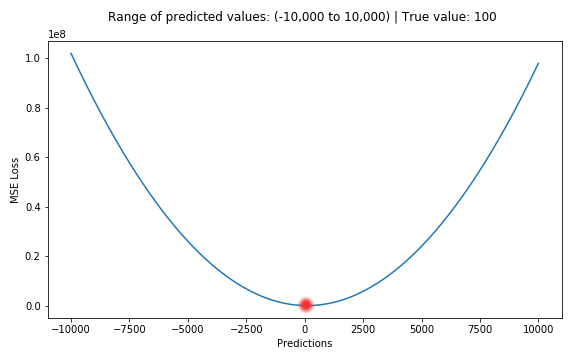
\includegraphics[width=0.85\textwidth]{figures/MSE_Loss.png}
    \caption{Regression Loss Function: Mean Squared Error (MSE). \\The horizontal axis represents the prediction error $(y - \hat{y})$, while the vertical axis represents the corresponding loss $(y - \hat{y})^2$.overestimation and underestimation are penalized equally. Furthermore, due to the quadratic nature of the loss, larger errors are penalized more strongly than smaller ones.}
    \label{fig:simulation_vs_AI}
\end{figure}

If the task involves predicting continuous values over time, this is referred to as a time-series forecasting problem. A typical example would be forecasting temperature in a thermal system. In this case, the input domain X could represent a sequence of past measurements, such as temperature, control inputs, or operating conditions over a fixed time window, and the target domain Y would consist of continuous values corresponding to future time steps. The training data would consist of multiple such sequences, each paired with the corresponding future value.

Generally, regression models aim to predict a single continuous value as the output. However, to account for uncertainty in predictions, the model can also be designed to output a range of possible values or a confidence interval instead of a single deterministic prediction.

\subsubsection{Classification}

Classification is a supervised learning task in which the objective is to assign an input to one of a finite set of predefined categories. In this setting, the target domain $\mathcal{Y}$ consists of discrete labels, and the model learns a mapping from input features to these labels based on labeled training data
In this setting, the target domain $\mathcal{Y}$ consists of discrete labels, typically defined as
\begin{equation}
\mathcal{Y} = \{1, 2, \dots, K\},
\end{equation}
where $K$ denotes the number of classes. The model learns a mapping function
\begin{equation}
f: \mathcal{X} \rightarrow \mathcal{Y},
\end{equation}
based on labeled training data, where $\mathcal{X}$ represents the input space.

In practice, many classification models output a probability distribution over the classes rather than a single label. This can be expressed as
\begin{equation}
\hat{y} = \left[ p(y = 1 \mid x), \dots, p(y = K \mid x) \right],
\end{equation}
where $p(y = k \mid x)$ denotes the predicted probability of input $x$ belonging to class $k$. The final class prediction is typically obtained by selecting the class with the highest probability.

A commonly used loss function for training classification models is the cross-entropy loss, defined as
\begin{equation}
\mathcal{L} = - \sum_{k=1}^{K} y_k \log \left( \hat{y}_k \right),
\end{equation}
which measures the discrepancy between the predicted probabilities and the true class labels. Classification methods are widely used in applications such as image recognition, spam detection, and fault diagnosis.    

\subsection{Activation Functions}

Activation functions are point-wise functions that define how neurons are activated or, colloquially, \textit{fire}. They are a crucial component of neural networks (NNs) because non-linear activation functions allow NNs to learn complex mappings that cannot be replicated through a sequence of linear operations. One of the most well-known activation functions is the sigmoid function (also referred to as the logistic function). Given an input $x$, the sigmoid activation is defined as:

\begin{equation}
\sigma(x) = \frac{1}{1 + e^{-x}}
\end{equation}

The resulting activation values range between 0 and 1, with values close to 0 corresponding to large negative inputs, and values approaching 1 corresponding to large positive inputs. The differentiability of the sigmoid function allows gradient descent during back-propagation to optimize the weights and biases within the network. Its derivative has an inverted-bell curve shape, reaching its maximum when $x = 0.5$.

When dealing with multi-class classification, the softmax function is typically applied in the last layer. The softmax function can be considered as a combination of multiple sigmoids and calculates relative probabilities. Similar to the sigmoid activation function, the softmax function returns the probability of each class:

\begin{equation}
\text{Softmax}(x_i) = \frac{\exp(x_i)}{\sum_j \exp(x_j)}
\end{equation}

In recent times, the Rectified Linear Unit (ReLU) has gained popularity due to its fast computation without any exponential component, as well as its ability to mitigate the vanishing gradient problem:

\begin{equation}
\text{ReLU}(x) = \max(0, x)
\end{equation}


\section{Random Forest Regressor}

Random Forest is an ensemble learning method that combines multiple decision trees to improve prediction robustness and reduce overfitting \cite{breiman2001random}. Each tree is trained on a bootstrapped subset of the training data (sampling with replacement), a technique known as bagging. Additionally, at each split, only a random subset of features is considered, which further decorrelates the trees and improves generalization.

Let the prediction of the $m$-th tree be given by
\begin{equation}
\hat{y}_m = h_m(x),
\end{equation}
where $h_m(\cdot)$ denotes the prediction function of the $m$-th decision tree.

The final Random Forest prediction is obtained by averaging the individual tree predictions:
\begin{equation}
\hat{y} = \frac{1}{M} \sum_{m=1}^{M} \hat{y}_m,
\end{equation}
where $M$ is the total number of trees in the ensemble.

During tree construction, splits are selected by maximizing the reduction in impurity. For regression tasks, impurity is typically measured using the variance of the target variable. The impurity at a node is defined as
\begin{equation}
I = \mathrm{Var}(Y) = \frac{1}{N} \sum_{i=1}^{N} (y_i - \bar{y})^2,
\end{equation}
where $\bar{y}$ is the mean of the target values in the node.

The impurity reduction achieved by a split is given by
\begin{equation}
\Delta I = I_{\text{parent}} - \sum_{k} \frac{N_k}{N} I_k,
\end{equation}
where $N_k$ is the number of samples in the $k$-th child node, $N$ is the number of samples in the parent node, and $I_k$ denotes the impurity of the child node.

An important property of Random Forests is their ability to estimate feature importance. A common measure is the mean decrease in impurity (MDI), computed as
\begin{equation}
\text{FI}(j) = \sum_{\text{splits on feature } j} \Delta I,
\end{equation}
which quantifies the contribution of feature $j$ to reducing prediction error across all trees.

\begin{figure}[H]
    \centering
    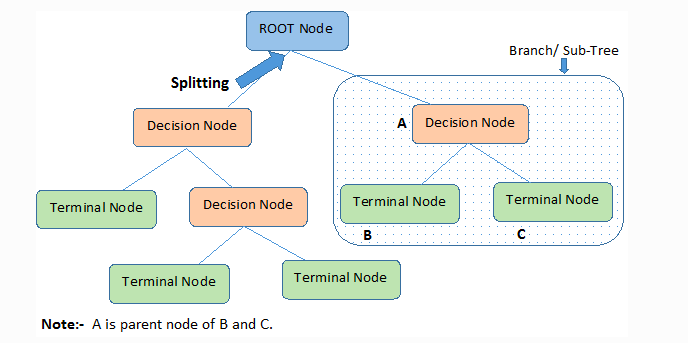
\includegraphics[width=0.85\textwidth]{figures/RandomForest.png}
    \caption{Structure of a Random Forest model showing multiple decision trees trained on bootstrapped datasets and aggregated via averaging.}
    \label{fig:Random Forest Tree}
\end{figure}

Random Forest regressors are attractive due to their interpretability, robustness to noise, and ability to capture complex nonlinear relationships. They also reduce variance compared to single decision trees while maintaining relatively low bias. In this thesis, Random Forest models are evaluated as baseline surrogate models and compared against neural network-based approaches.

\section{Principal Component Analysis (PCA)}

Principal Component Analysis (PCA) is a statistical technique used to reduce the dimensionality of data while preserving most of its variance. In many engineering applications, including thermal system modeling, datasets often contain highly correlated features. This is particularly relevant for time-series outputs such as temperature or energy evolution, where adjacent time steps exhibit strong correlation. High-dimensional data increases computational cost and may negatively affect the performance and generalization capability of machine learning models.

Let the dataset be represented by a matrix
\begin{equation}
\mathbf{X} \in \mathbf{R}^{N \times D},
\end{equation}
where $N$ denotes the number of samples and $D$ denotes the number of features. PCA begins by centering the data:
\begin{equation}
\mathbf{X}_c = \mathbf{X} - \bar{\mathbf{X}},
\end{equation}
where $\bar{\mathbf{X}}$ represents the mean of each feature.

The covariance matrix of the centered data is then computed as
\begin{equation}
\mathbf{\Sigma} = \frac{1}{N-1} \mathbf{X}_c^T \mathbf{X}_c.
\end{equation}

Eigenvalue decomposition of the covariance matrix yields a set of eigenvectors and corresponding eigenvalues:
\begin{equation}
\mathbf{\Sigma} \mathbf{w}_i = \lambda_i \mathbf{w}_i,
\end{equation}
where $\lambda_i$ represents the variance explained by the $i$-th principal component, and $\mathbf{w}_i$ is the corresponding eigenvector.

The principal components are obtained by projecting the data onto the subspace spanned by the eigenvectors associated with the largest eigenvalues:
\begin{equation}
\mathbf{Z} = \mathbf{X}_c \mathbf{W}_K,
\end{equation}
where $\mathbf{W}_K \in \mathbf{R}^{D \times K}$ contains the top $K$ eigenvectors. This results in a reduced representation $\mathbf{Z} \in \mathbf{R}^{N \times K}$.

The proportion of variance explained by the selected components is given by
\begin{equation}
\frac{\sum_{i=1}^{K} \lambda_i}{\sum_{i=1}^{D} \lambda_i}.
\end{equation}

The number of retained components $K$ is typically chosen such that a predefined percentage of the total variance, commonly between 95\% and 99\%, is preserved.
 
\begin{figure}[H]
    \centering
    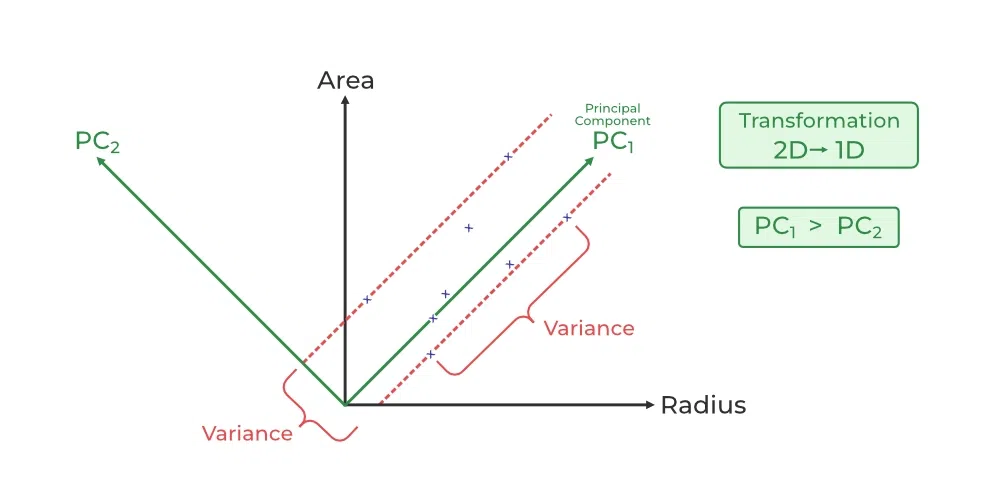
\includegraphics[width=0.85\textwidth]{figures/Principal_Componenent_Analysis.png}
    \caption{Projection of data onto principal components, where the first component captures the maximum variance.}
    \label{fig:Random Forest Tree}
\end{figure}

In this thesis, PCA is applied to the time-series outputs generated by the Dymola thermal model. Instead of directly predicting high-dimensional thermal signals, the surrogate models are trained to predict the reduced set of PCA coefficients. The original time-series outputs are subsequently reconstructed using the inverse PCA transformation:
\begin{equation}
\mathbf{X} \approx \mathbf{Z} \mathbf{W}_K^T + \bar{\mathbf{X}}.
\end{equation}

This approach significantly reduces computational complexity, improves training stability, and removes redundancy in the thermal data while preserving the essential system behavior.

% \section{PRINCIPAL COMPONENT ANALYSIS (PCA)}

% Principal Component Analysis (PCA) is a statistical technique used to reduce the dimensionality of data while preserving most of its variability. In many engineering applications, including thermal system modeling, datasets often contain highly correlated features. This is particularly true for time-series outputs such as battery temperature or energy evolution, where adjacent time steps exhibit strong correlation. High-dimensional data increases computational cost and may negatively impact the performance and generalization capability of machine learning models.

% Let the dataset be represented by a matrix
% \[
% \mathbf{X} \in \mathbb{R}^{N \times D},
% \]
% where \( N \) denotes the number of samples and \( D \) denotes the number of features. PCA first centers the data by subtracting the mean of each feature. The covariance matrix is then computed as:
% \[
% \boldsymbol{\Sigma} = \frac{1}{N-1} \mathbf{X}^\top \mathbf{X}.
% \]

% Eigenvalue decomposition of the covariance matrix yields a set of eigenvectors and corresponding eigenvalues. The eigenvectors define the principal components, while the eigenvalues indicate the amount of variance captured by each component. By selecting only the first \( K \) principal components associated with the largest eigenvalues, the data can be projected onto a lower-dimensional subspace:
% \[
% \mathbf{Z} = \mathbf{X} \mathbf{W}_K,
% \]
% where \( \mathbf{W}_K \in \mathbb{R}^{D \times K} \) contains the eigenvectors corresponding to the \( K \) largest eigenvalues.

% The number of retained components is typically chosen such that a predefined percentage of the total variance, commonly between 95\% and 99\%, is preserved.

% In this thesis, PCA is applied to the time-series outputs generated by the Dymola thermal model. Instead of directly predicting high-dimensional thermal signals, the surrogate models are trained to predict the reduced set of PCA coefficients. The original time-series outputs are subsequently reconstructed using the inverse PCA transformation. This approach significantly reduces computational complexity, improves training stability, and removes redundancy in the thermal data while preserving the essential thermal system behavior.



\section{Data Splitting}

In supervised learning, if all available data observations are used as a training set to fit the model, the challenge of selecting appropriate hyperparameters remains. The ultimate goal is not only to fit the observed data but also to generalize well to new, unseen data. 

To evaluate the model's ability to generalize after training and to select the best hyperparameters, the dataset is typically divided into randomly chosen subsets: training, validation, and test sets.

\begin{itemize}
    \item The \textbf{training set} is used to learn model parameters.
    \item The \textbf{validation set} is used to tune hyperparameters by comparing predictions with actual outcomes.
    \item The \textbf{test set} is used to evaluate the final model performance on unseen data.
\end{itemize}

After identifying the optimal hyperparameters and achieving satisfactory validation performance, the model is assessed on the test set. The exact proportions of these splits, often referred to as \textit{data-split}, depend on the specific model and dataset size. A commonly used empirical split is:

\begin{equation}
70\% \text{ (training)}, \quad 10\% \text{ (validation)}, \quad 20\% \text{ (test)}
\end{equation}

These neural networks are widely utilized in many applications, with autonomous driving being a prominent example. In this work, the focus is particularly on object detection.

\section{Model evaluation}

Model performance is evaluated using quantitative metrics, including:
\begin{itemize}
    \item Mean Squared Error (MSE)
    \item Coefficient of Determination (\( R^2 \))
\end{itemize}

The coefficient of determination is defined as:

\[
\mathrm{MSE} = \frac{1}{N} \sum_{i=1}^{N} \left( y_i - \hat{y}_i \right)^2.
\]

\[
R^2 = 1 - \frac{\sum_{i=1}^{N} \left( y_i - \hat{y}_i \right)^2}
{\sum_{i=1}^{N} \left( y_i - \bar{y} \right)^2},
\]
where
\[
\bar{y} = \frac{1}{N} \sum_{i=1}^{N} y_i
\]
denotes the mean of the ground truth values.

In addition to prediction accuracy, computational efficiency is assessed by comparing the model prediction time against the numerical simulation time. This evaluation directly reflects the primary objective of this thesis, namely reducing computational cost while maintaining high predictive fidelity.
